% !TEX root = dissertation_BB.tex
%% spellcheck-language en-US

%    #
%   #
%  #  #
%  #####
%     #

\chapter{Real-time, GPU accelerated image processing pipeline}

\graphicspath{{./figures/4_gpu/}}


\section{Challenges in data handling for light-sheet microscopy}

  When using any kind of microscopy in research, image processing is a crucial part of the workflow. This is especially true for light-sheet microscopy, since it is capable of imaging the same specimen for multiple days, producing immense amounts of data. A single overnight experiment of \textit{Drosophila} development (which is a very typical use-case for light-sheet) can produce multiple terabytes of data.

  Apart from light-sheet microscopy, many other microscopy modalities are also suffering from this problem. Methods, such as high content screening \cite{carpenter_systematic_2004,echeverri_high-throughput_2006,pepperkok_high-throughput_2006}, where tens of thousands of different genotypes are imaged generating millions of images; and single molecule localization microscope (SMLM) \cite{betzig_imaging_2006,hess_ultra-high_2006,rust_sub-diffraction-limit_2006}, where just a single plane of a single sample is imaged hundreds of thousands of times to acquire super-resolved images.

  Not only these methods are capable of generating data extremely fast, but with the sustained high data rate a single experiment can easily reach multiples of terabytes (\autoref{fig:sizes}). Handling this amount of data can quickly become the bottleneck for many discoveries, which is a more and more common issue in biological research \cite{wollman_high_2007,reynaud_guide_2015,perkel_struggle_2016}. 


  \begin{figure}[btp]
    \centering
    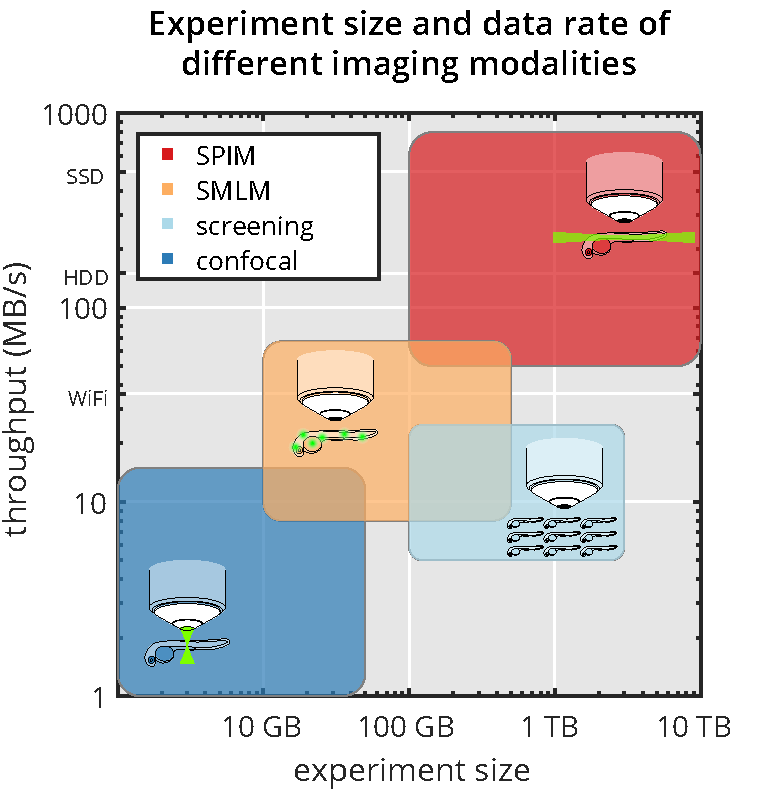
\includegraphics[page=1,width=0.5\textwidth]{comparison_with_pictograms}
    \bcaption[Experiment sizes and data rate of different imaging modalities]{Comparison of single-plane illumination microscopy (SPIM, red rectangle), high-content screening (light blue), single molecule localization microscopy (SMLM, orange) and confocal microscopy (blue) by typical experiment size and data production rate (see also Table \ref{tab:sizes}).}
    \label{fig:sizes}
  \end{figure}

  % To efficiently and quickly process such amounts of information, developing new strategies / innovative approaches is indispensible. As image processing tasks are typically highly parallelizable 

  This chapter will focus on addressing these challenges, by presenting a real-time, GPU-based image preprocessing pipeline consisting of two parts (\autoref{fig:pipeline}).
  The first part is a fast image fusion method for our workhorse light-sheet microscope, the MuVi-SPIM \cite{krzic_multiview_2012}, that enables live fusion of the images arriving from two opposing cameras.
  The second part of the pipeline, which can also be used in a standalone way, is a real-time image compression library that allows lossless and noise dependent lossy compression of the data already during acquisition.

  \begin{figure}
    \centering
    \includegraphics[width=\textwidth]{pipeline}
    \bcaption[Real-time image processing pipeline for multi-view light-sheet microscopy]{}
    \label{fig:pipeline}
  \end{figure}



  \section{CUDA architecture}

    CUDA \cite{nickolls_scalable_2008}
    CUDA programming Guide \cite{nvidia_cuda_2015}



    % ######## ##     ##  ######  ####  #######  ##    ## 
    % ##       ##     ## ##    ##  ##  ##     ## ###   ## 
    % ##       ##     ## ##        ##  ##     ## ####  ## 
    % ######   ##     ##  ######   ##  ##     ## ## ## ## 
    % ##       ##     ##       ##  ##  ##     ## ##  #### 
    % ##       ##     ## ##    ##  ##  ##     ## ##   ### 
    % ##        #######   ######  ####  #######  ##    ## 

\section{Live fusion}

Similarly to the DualMouse-SPIM, our currently used production microscope, the Multiview-SPIM (MuVi-SPIM) \cite{krzic_multiview_2012} also uses multiple imaging directions to improve the image quality. In this case, however, the aim is completeness rather than increasing the resolution. As the MuVi-SPIM is capable of imaging much larger specimens, such as entire \textit{Drosophila} embryos, the sample size itself can present some challenges, especially for opaques specimens. As light scattering and absorption impacts both the illumination and detection optics, the negative effects for SPIM are more pronounced compared to single-lens systems \cite{de_medeiros_deep_2016}.




\subsection{Multiview SPIM for \textit{in toto} imaging}

MuVi-SPIM  provides an elegant solution for multi-view imaging. A standard SPIM setup with a single detection and a single illumination lens would rotate the sample to acquire images from multiple directions. MuVi-SPIM, on the other hand, utilizes two opposing objectives for illumination, and two opposing objectives for detection (\autoref{fig:muvi-spim}a). As the sample is held by an aqueous gel inside the imaging chamber, all objectives have unobstructed view of it from multiple directions (\autoref{fig:muvi-spim}b,c).

Data acquisition is done in two steps: the sample is illuminated by Light sheet 1, and fluorescence is collected by both detection objectives at the same time, after which Light sheet 2 is activated, and both cameras record the fluorescence again (\autoref{fig:muvi-spim}d). This process will result in 4 datasets, all with partial information due to scattering effects. The 4 views are later fused to a single, high quality dataset (\autoref{fig:muvi-spim}e). This fusion process is necessary before any further analysis steps can be performed, however, due to the sheer size of the data, it takes a considerable amount of time after the acquisition.

By combining scanned light-sheet \cite{keller_reconstruction_2008} with confocal slit detection on the camera chip \cite{baumgart_scanned_2012}, it is possible to exclude out of focus, scattered illumination light. This way it is  possible to illuminate simultaneously with both light-sheets, which leaves us with only two views, the views of the two opposing cameras \cite{de_medeiros_confocal_2015}.

\begin{figure}
  \centering
  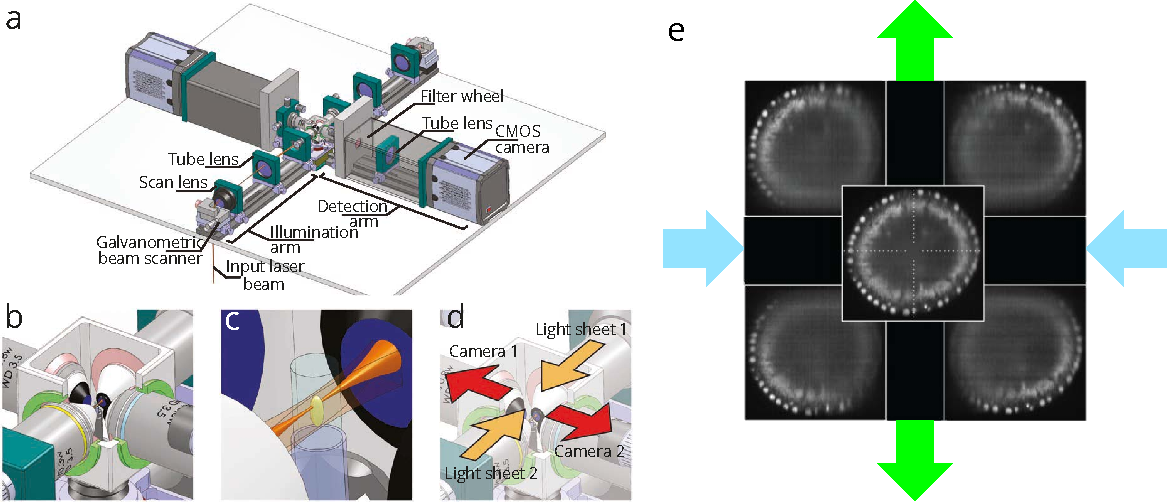
\includegraphics[width=1\columnwidth]{fusion/muvi-spim}
  \bcaption[Operating principle of MuVi-SPIM]{(a) The microscope consists of two illumination and two detection arms for simultaneous multi-view illumination and detection. (b) The 4 arms meet in the imaging chamber that is filled with water, and contains the sample. (c) The sample is held by a glass capillary, in  a GelRite cylinder. Optical sectioning is acheived by a virtaul light-sheet. (d) The light-sheets can be generated from two sides (Light sheet 1 and 2), and detection is also double sided (Camera 1 and 2). Adapted from \cite{krzic_multiview_2012}.}
  \label{fig:muvi-spim}
\end{figure}




\subsection{Image registration}

To perform image fusion of multiple views, first image registration is necessary: the coordinate systems of both views have to be properly overlapped. Ideally a single mirroring transformation would be enough to superpose the two camera images, however in practice the microscope can never be aligned with such precision. Other types of transformations are also necessary: translation to account for offsets in the field of view; scaling in case of slightly different magnifications; and also shearing if the detection plane is not perfectly perpendicular to the sample movement direction \cite{krzic_multiple-view_2009}. To combine all of these effects, a full, 3D affine transformation is necessary to properly align the two camera images (Fig. \ref{fig:acquisition} a). This transformation can be represented by a matrix multiplication with 12 different parameters:
\[
\begin{pmatrix}
a & b & c & d \\ 
e & f & g & h \\ 
i & j & k & l \\
0 & 0 & 0 & 1 
\end{pmatrix}
\times
\begin{pmatrix}
x\\
y\\
z\\
1
\end{pmatrix}
=
\begin{pmatrix}
a x + b y + c z + d\\ 
e x + f y + g z + g\\ 
i x + j y + k z + l\\
1
\end{pmatrix}
\]
where $x, y, z$ are the coordinates of the original 3D image, and $a, b, ..., l$ are the affine transformation parameters.

These parameters are traditionally acquired by a bead based registration algorithm after imaging fluorescent beads from each view of the microscope \cite{preibisch_bead-based_2009,preibisch_software_2010}. The beads are segmented by using a difference of Gaussian filter, and the registration parameters are acquired by matching the segmented bead coordinates in each view. Identifying the corresponding beads in each view is done by a translation and rotation invariant local geometric descriptor. This matches the beads based on their relative position to their nearest neighbors. After the matching beads are identified, the affine transformation parameters are calculated by minimizing the global displacement for each pair of beads.

For the two opposing views of MuVi-SPIM, these parameters are only dependent on the optical setup itself, and not the sample or the experiment. Because of this, it is sufficient to determine the transformation parameters only after modifying the microscope (\textit{e.g.} after realignment).

In our previous fusion pipeline, after the parameters were acquired, the 3D stacks are fused by transforming one of the views to the coordinate system of the other (using the affine transformation parameters from the bead based registration), and fusing the two stack by applying a sigmoidal weighted average. The weights are determined in a way to exclude the parts of a stack that has worse image quality, and complement is from the other view. When using the electronic confocal slit detection (eCSD) weighting is not necessary, as the scattered light is already rejected in these recordings, and a simple sum of the two stacks gives the best results regardless of the sample \cite{de_medeiros_confocal_2015}.

The fusion process itself, can be very resource intensive, and take a considerable amount of time. This is simply due to the size of the 3D stacks: a single stack is usually between 2 and \SI{4}{GB} in size. Thus, the necessary memory requirement to fuse 2 of these stacks is $3\cdot \SI{4}{GB} = \SI{12}{GB}$, as the result will also take up the same space. Just reading and writing this amount of information to the hard disk takes a considerable amount of time. When using an SSD drive for example, with a \SI{500}{MB/s} read/write speed, just the I/O operations will take around $\frac{\SI{12}{GB}}{\SI{500}{MB/s}} = \SI{24}{s}$.


\begin{figure}
  \centering
  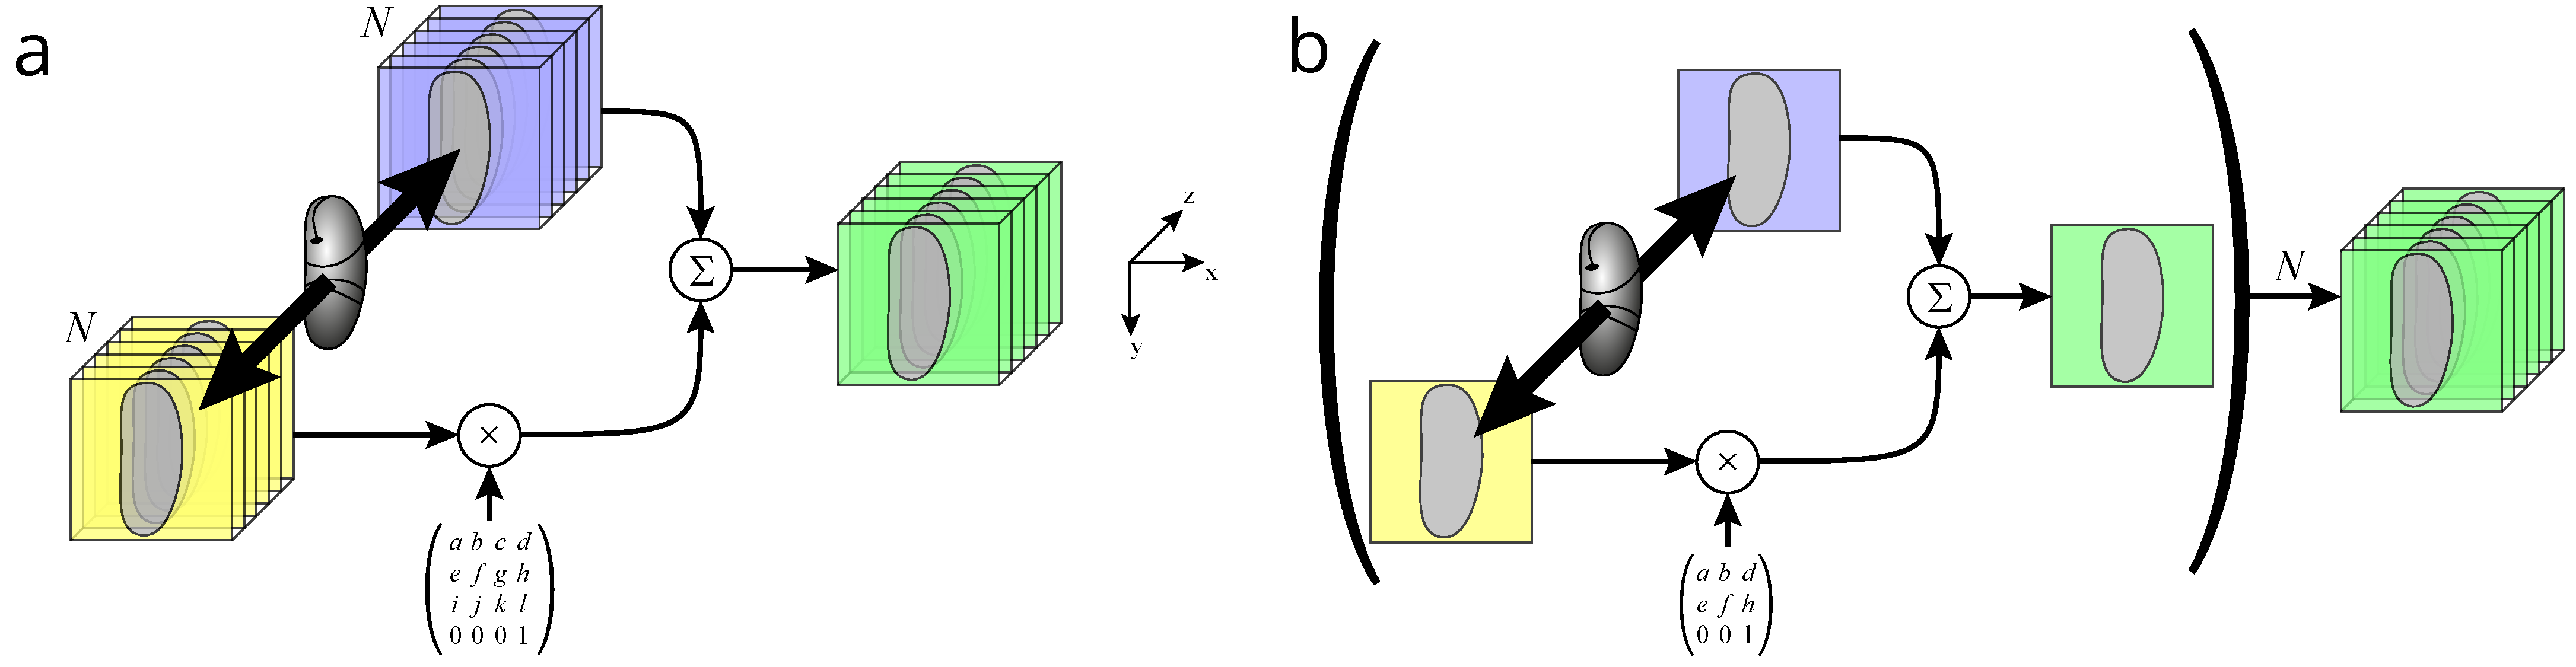
\includegraphics[width=1\columnwidth]{fusion/acquisition}
  \bcaption[Multi-view fusion methods for light-sheet microscopy]{a) Full 3D stacks are acquired from the opposing views (yellow and blue), which are then registered in 3D space using previously acquired affine transformation parameters. Registered stacks are then weighted averaged to create the final fused stack (green). b) Images from opposing views are directly fused plane by plane. Registration takes place in 2D space thus reducing computational effort and memory requirements. The registered planes are then weighted averaged to create the final fused image.}
  \label{fig:acquisition}
\end{figure}

It would be much more practical to already fuse the opposing views before displaying or saving the image. Since the two cameras ideally image the same $z$ plane, it should be possible to reduce the alignment problem to a 2D affine transformation:
\[
\begin{pmatrix}
a & b & d\\ 
e & f & h \\
0 & 0 & 1
\end{pmatrix}
\times
\begin{pmatrix}
x\\
y\\
1
\end{pmatrix}
=
\begin{pmatrix}
a x + b y + d\\ 
e x + f y + g\\
1
\end{pmatrix}
\]
If this is possible, then fusion can be carried out separately for each image plane (Fig. \ref{fig:acquisition} b), which would greatly facilitate live image fusion. The requirements for this are the following:
\begin{align}
\left| c z \right| &< \sigma_{xy} & \forall z \label{eq:req1}\\
\left| g z \right|  &< \sigma_{xy} & \forall z \label{eq:req2}\\
\left| i x + j y + (k-1)  z + l \right| &< \sigma_z & \forall x, y, z  \label{eq:req3}
\end{align}
where $\sigma_{xy}$ is the lateral resolution, and $\sigma_z$ is the axial resolution of the microscope, which are 277 nm and 1099 nm respectively. 

 If these conditions hold (\textit{i.e.} the microscope is properly aligned), then direct plane by plane fusion will not result in any loss of information compared to the full 3D image fusion.

% \subsection{Image preprocessing pipeline}

% \begin{figure}[bth]
% \centering
% \includegraphics[width=0.4\columnwidth]{fusion/pipeline}
% \caption{Image preprocessing pipeline. The pipeline comprises of two parts: processing on CPU (white background) and processing on GPU (green background). Images are first transferred from the CPU to the GPU, where the preprocessing steps take place. These include background subtraction, affine transformation, weighted averaging and optionally thumbnail generation and image compression. After the preprocessing steps the image is transferred back to the CPU, and saved on the hard drive, or streamed to a remote computer. Data sizes after each preprocessing step are shown in the gray bands for planes, stacks and time-lapses.}
% \label{fig:pipeline}
% \end{figure}

% To perform the image fusion step as fast as possible, thus enabling it is use for live imaging, we used CUDA (Compute Unified Device Architecture) \cite{_cuda_????-1} to implement the algorithm on a graphics card (NVIDIA, GTX 750). This architecture offers a convenient way to harness the massively parallel computing capabilities of the many streaming multiprocessors residing on a GPU (graphics processing unit). Since each processing step we require is pixel based, they can be inherently parallelized to gain tremendous advantage in computing time.

% To utilize the GPU for the image processing step, the images first have to be transferred from the computer main memory to the graphics card memory. Because of the limited bandwidth of the PCIe 2.0 16x bus, this step is actually the bottleneck, and not the computation itself. To optimize data transfer speed, several techniques can be used.

% First, one has to make sure that the space for the original image data is allocated as paged-lock memory. This is possible with \texttt{cudaMallocHost}. This function will make sure that the memory space allocated on the host will be page-locked \textit{i.e.} it is contents cannot be temporarily swapped to the pagefile on the hard disk, and it is actually mapped to the physical memory. Otherwise, with normal allocation functions this is not guaranteed by the operating system, and the memory is only mapped to the physical memory when it is contents are accessed, which heavily influence read/write speed.

% Second, if the same operation is carried out for many images (as in the case of our live fusion method), the data transfer for the next image can already be carried out while the previous image is being processed, thus masking at least one of the data transfers between the main memory and the graphics card.

% % Even when using both methods, most of the time is still taken by the data transfer. Because of this, we decided to implement additional image preprocessing steps in our pipeline (Fig \ref{fig:pipeline}, thus ...

% %To maximize GPU utilization, and ultimately justify the long data transfer times, in addition to the plane by plane fusion (which is actually an affine transformation followed by weighted average), we also implemented background subtraction, subsampling, LUT conversion from 16 bits to 8 bits, and JPEG compression in our pipeline (Fig \ref{fig:pipeline}). All of these steps either enhance image quality (such as background subtraction), reduce data size (LUT conversion, subsampling, JPEG), or both (fusion).

% Since our microscope control software is implemented in LabVIEW, all the functions in our pipeline were incorporated in a dynamic linked library (DLL) which can be loaded by LabVIEW to use the CUDA functions. Furthermore, to facilitate the integration to existing software, we created a LabVIEW library based on these CUDA functions, to provide a consistent and easy to use interface for further development.

\subsection{CUDA implementation of direct fusion}
  As our custom microscope control software (\autoref{sec:software}) is implemented in LabVIEW, we implemented the pipeline as a combination of a CUDA and a LabVIEW library. The CUDA library implements all the necessary low level functions, and exposes these in a dynamically linked library (dll). The LabVIEW library, \texttt{LVCUDA.lvlib} implements two high level classes: \texttt{cuArray}, and \texttt{Texture} (\autoref{fig:LVCUDA}). These interface to the CUDA dll, and allow to easily build a flexible CUDA-based image processing pipeline in LabVIEW.

  \begin{figure}
    \centering
    \begin{subfigure}[t]{0.49\textwidth}
      \centering
      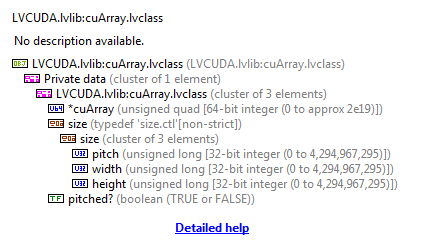
\includegraphics[width=\textwidth]{fusion/CuArray}
      \caption{}
    \end{subfigure}
    \begin{subfigure}[t]{0.49\textwidth}
      \centering
      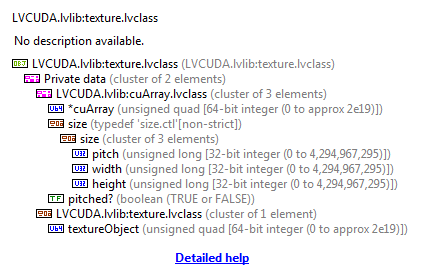
\includegraphics[width=\textwidth]{fusion/Texture}
      \caption{}
    \end{subfigure}
    \bcaption[Classes of LVCUDA library]{(a) \texttt{CuArray} class, wrapping a 1D or 2D pitched device memory for use in LabVIEW. (b) \texttt{Texture} class, wrapping a CUDA texture object for use in LabVIEW.}
    \label{fig:LVCUDA}
  \end{figure}

  \subsubsection{\texttt{cuArray} LabVIEW class}

  \subsubsection{\texttt{Texture} LabVIEW class}

\subsection{Results}

  \begin{figure*}[tb]
    \centering
    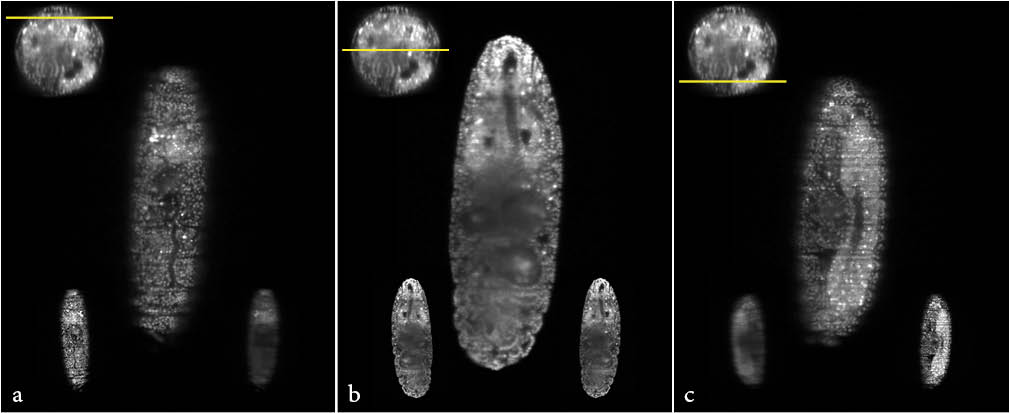
\includegraphics[width=1\textwidth]{fusion/drosophila_D2}
    \caption{ GPU fused images of a \textit{Drosophila melanogaster} embryo. Two stacks were taken in quick succession first without fusion, then with fusion enabled. Fused images are shown in the middle of each subfigure, while the individual camera images are in the bottom insets. The top-left inset depicts the z-position of the shown images. a) Image from closer to the left camera. b) Image from the center of the embryo. c) Image from closer to the right camera.}
    \label{fig:drosophila}
  \end{figure*}

  The image preprocessing pipeline was tested on our previously described Multi-View Single Plane Illumination Microscope (MuVi-SPIM)\cite{krzic_multiview_2012}. For the background subtraction we recorded 1500 dark images with each camera and averaged them, to obtain the camera specific background images. Before image acquisition these were uploaded to the GPU memory, and were readily available for the pipeline.

  After careful alignment of the microscope to meet the previously discussed requirements (Eqs. \eqref{eq:req1} -- \eqref{eq:req3}), we imaged fluorescent beads in a gel suspension to obtain the affine transformation parameters. After making sure that these parameters indeed fulfill the previously set requirements, these were also uploaded to the GPU memory for further use in our pipeline.

  To validate our hypotheses, that 2D direct image fusion is sufficient instead of the full 3D fusion, we image several samples. First, we imaged the flourescent beads again, now with the live fusion enabled, to make sure our registration parameters are correct. Manual evaluation of the data revealed that the fusion indeed worked, without any artifacts, such as double beads which would indicate an imprecision in alignment or in the transformation parameters.

  We also applied the live fusion to a real biological specimen, namely \textit{Drosophila melanogaster} embryos expressing H2Av-mCherry histone marker. The embryos were imaged first without direct fusion enabled, and immediately afterwards with direct fusion enabled (Fig. \ref{fig:drosophila}). Image quality dependency on the depth of the imaging plane is especially apparent in single-view stacks. Planes closer to the camera give a sharp, high contrast image, while planes further then the middle of the embryo are severely degraded due to scattering.

  Stacks obtained with the live fusion enabled show a consistently high image quality throughout the entire stack, independent of the depth. This allows us to keep only the already fused data, thus effectively reducing the storage requirement by half, and facilitating further data processing steps. 


% \section{Conclusions}

% I developed a direct plane by plane fusion method which was implemented in CUDA, and can be performed live, directly on the microscope. This results in a single, high quality recording, which can be directly used later for further processing or data evaluation. We showed the viability of the method by imaging fluorescent beads, and fluorescently labeled \textit{Drosophila m.} embryos, which showed superior image quality to both of the original views. As a further consequence, data handling became easier, less storage is needed for further experiments, and considerable time is spared by eliminating the need for the 3D fusion step.

% For several samples orthogonal views are desired, or in some cases the optical setup is already designed with orthogonal detection\cite{wu_spatially_2013}, or close to orthogonal in the case of the symmetric mouse SPIM. In these cases to properly fuse the different directions, multi-view deconvolution is necessary \cite{krzic_multiple-view_2009,temerinac-ott_multiview_2012} to gain maximum information from both views.






%#######   #######  ########  
%#     ## ##     ## ##     ## 
%#     ##        ## ##     ## 
%#######   #######  ##     ## 
%#     ##        ## ##     ## 
%#     ## ##     ## ##     ## 
%#######   #######  ########  
  
\section{\b3d image compression}

  The second part of our GPU-based image preprocessing pipeline is a new image compression algorithm that allows for extremely fast image compression to efficiently reduce data sizes already during acquisition.
  
  

  A straightforward solution to these problems would be to compress the images during acquisition. Although this would not reduce the requirements for image processing power and time, it still has a big impact on the necessary background infrastructure. By reducing the data size, not only the cost for storage can be reduced, but the time it takes to transfer the data during the various steps of data processing. A fast compression method would also greatly improve 3D data browsing possibilities, as more data could be piped to the rendering software.

  Despite these advantages, not many microscopists have implemented real time compression strategies during acquisition, and this is mostly due to the lack of appropriate compression methods suitable for scientific imaging that also offers the high throughput demanded by these applications. Typically used lossless compression methods, such as JPEG2000 \cite{adams_jpeg-2000_2001} although offer good compression ratios, are very slow in processing speed, at least compared to the data rate of a modern microscope ($\sim \SI{1}{GB/s}$). High speed compression methods that could deal with this data rate have been developed for ultra high definition 4K and 8K digital cameras, such as the high efficiency video codec (HEVC) \cite{international_telecommunications_union_h.265_2016}. These methods, however, have been optimized for lossy image compression which is generally not acceptable for scientific data \cite{cromey_digital_2013}, and rarely support compression of high bit rate originals, which is typically the case for modern sCMOS sensors. Although the HEVC recommendation does specify bit rates up to 16 bits, and lossless compression, we

  To address these issues, we developed \b3d, a GPU based image compression method that is capable of high speed compression of microscopy images during the image acquisition process. By utilizing the massively parallel processing architecture of a GPU, we were not only able to reach a compression and decompression speed of \SI{1}{GB/s}, but our algorithm also keeps the load off the CPU, making it available for other computing tasks related to operating the microscope itself.

  A second feature of our compression library is a novel algorithm for noise dependent lossy compression of scientific images. As mentioned before, lossy compression is not recommended for scientific images, and the reason for this, is all practical lossy compression algorithms are designed with the intent of fooling the human visual system \cite{sayood_introduction_2012}. While the images compressed by these algorithms may appear identical to the eye, any downstream data analysis could be negatively impacted by the compression artifacts. To our knowledge, only a single algorithm allows to set the loss in a deterministic manner: the near-lossless operating mode of JPEG-LS \cite{weinberger_loco-i_2000}. In this mode it is possible to set the maximum allowable error a pixel can have after decompression. Although this can be useful for certain applications, it has not been widely implemented, as the visual quality loss is more severe compared to other algorithms with the same compression ratio \cite{santa-cruz_study_2000}.

  \b3d image compression
  light-sheet (Sec. \ref{sec:light-sheet})
  data handling is bottleneck 

  KLB \cite{amat_efficient_2015}

  big data viewer \cite{pietzsch_bigdataviewer:_2015}
  Fiji \cite{schindelin_fiji:_2012}

  FLIC \cite{wang_fast_2012}
  SFALIC \cite{starosolski_simple_2007}
  FELICS \cite{howard_fast_1993} -> this was before JPEG-LS
  Treib terrain editing \cite{treib_interactive_2012}
  Treib turbulence \cite{treib_turbulence_2012}



    


    

  \subsection{Compression algorithm}

    compression scheme: modeling+ coding \cite{rissanen_universal_1981}

    \begin{figure}[tpb]
      \centering
      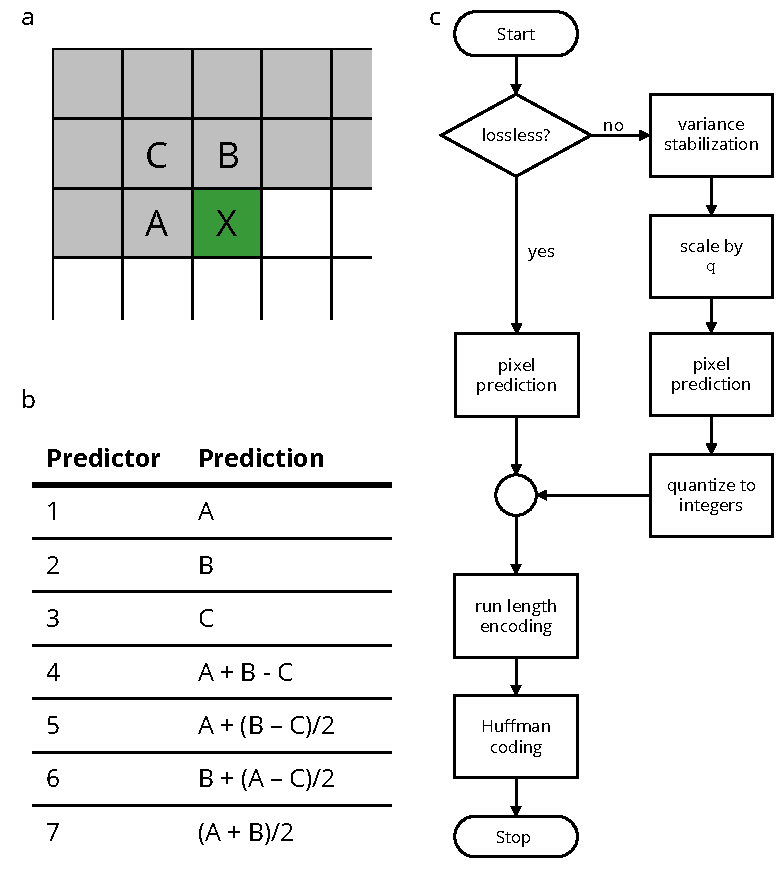
\includegraphics[page=1,width=0.6\textwidth]{SFig1_flow}
      \bcaption[\b3d algorithm schematics]{(\textbf{a}) Prediction context for pixel X, the next sample to be encoded. Three neighboring pixels are considered: left (A), top (B) and top left (C) neighbors. (\textbf{b}) Lossless JPEG predictors for X, based on the context showed in (\textbf{a}). The first three predictors are one-dimensional, while the rest are two-dimensional. Using a two dimensional predictor while increases complexity slightly, also increases the achievable compression ratio. We found that for fluorescence microscopy images predictor 7 performs best, hence its inclusion in the \b3d algorithm. (\textbf{c)} Complete algorithm flowchart depicting the main stages of the compression. First, if the result should be lossless, pixel prediction is performed on the original image values. If within noise level mode is selected, the image noise is stabilized first (see "\textbf{Supplementary Note}"), which is then scaled by the quantization step q. Prediction is performed, and the prediction errors are rounded to the nearest integer. The prediction errors for both lossless and lossy modes are then run-length encoded, and finally Huffman coding is applied to effectively reduce data size. The output of the Huffman coder is saved as the compressed file.}
      \label{fig:algorithm}
    \end{figure}



    \begin{figure}[tpb]
      \centering
      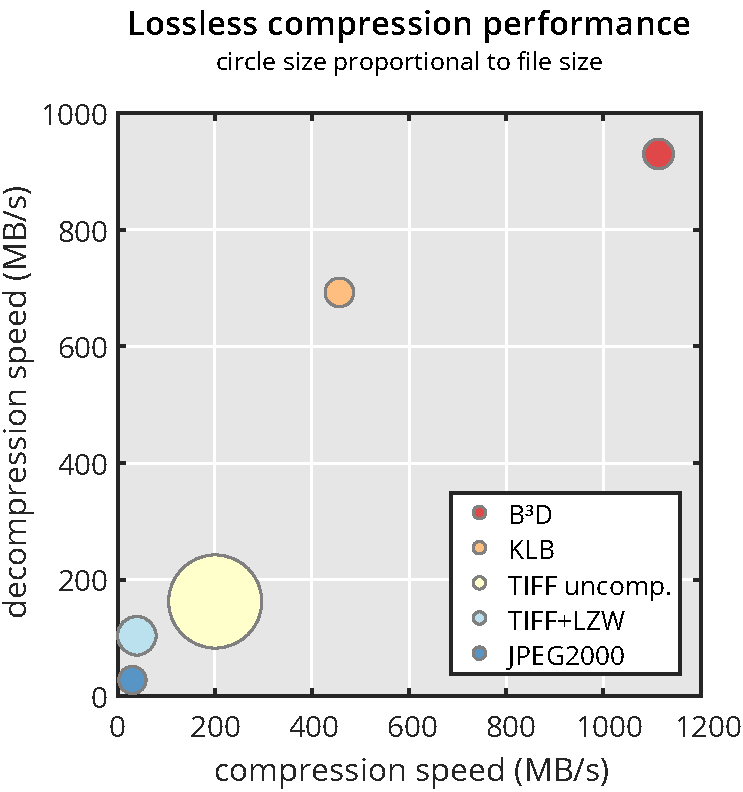
\includegraphics[page=1,height=0.5\textwidth]{bubbles}
      \bcaption[Lossless compression performance]{Performance comparison of our \b3d compression algorithm (red circle) vs. KLB (orange), uncompressed TIFF (light yellow), LZW compressed TIFF (light blue) and JPEG2000 (blue) regarding write speed (horizontal axis), read speed (vertical axis) and file size (circle size). (see also Table \ref{tab:performance}).}
      \label{fig:performance}
    \end{figure}

    

    \begin{figure}[tpb]
      \centering
      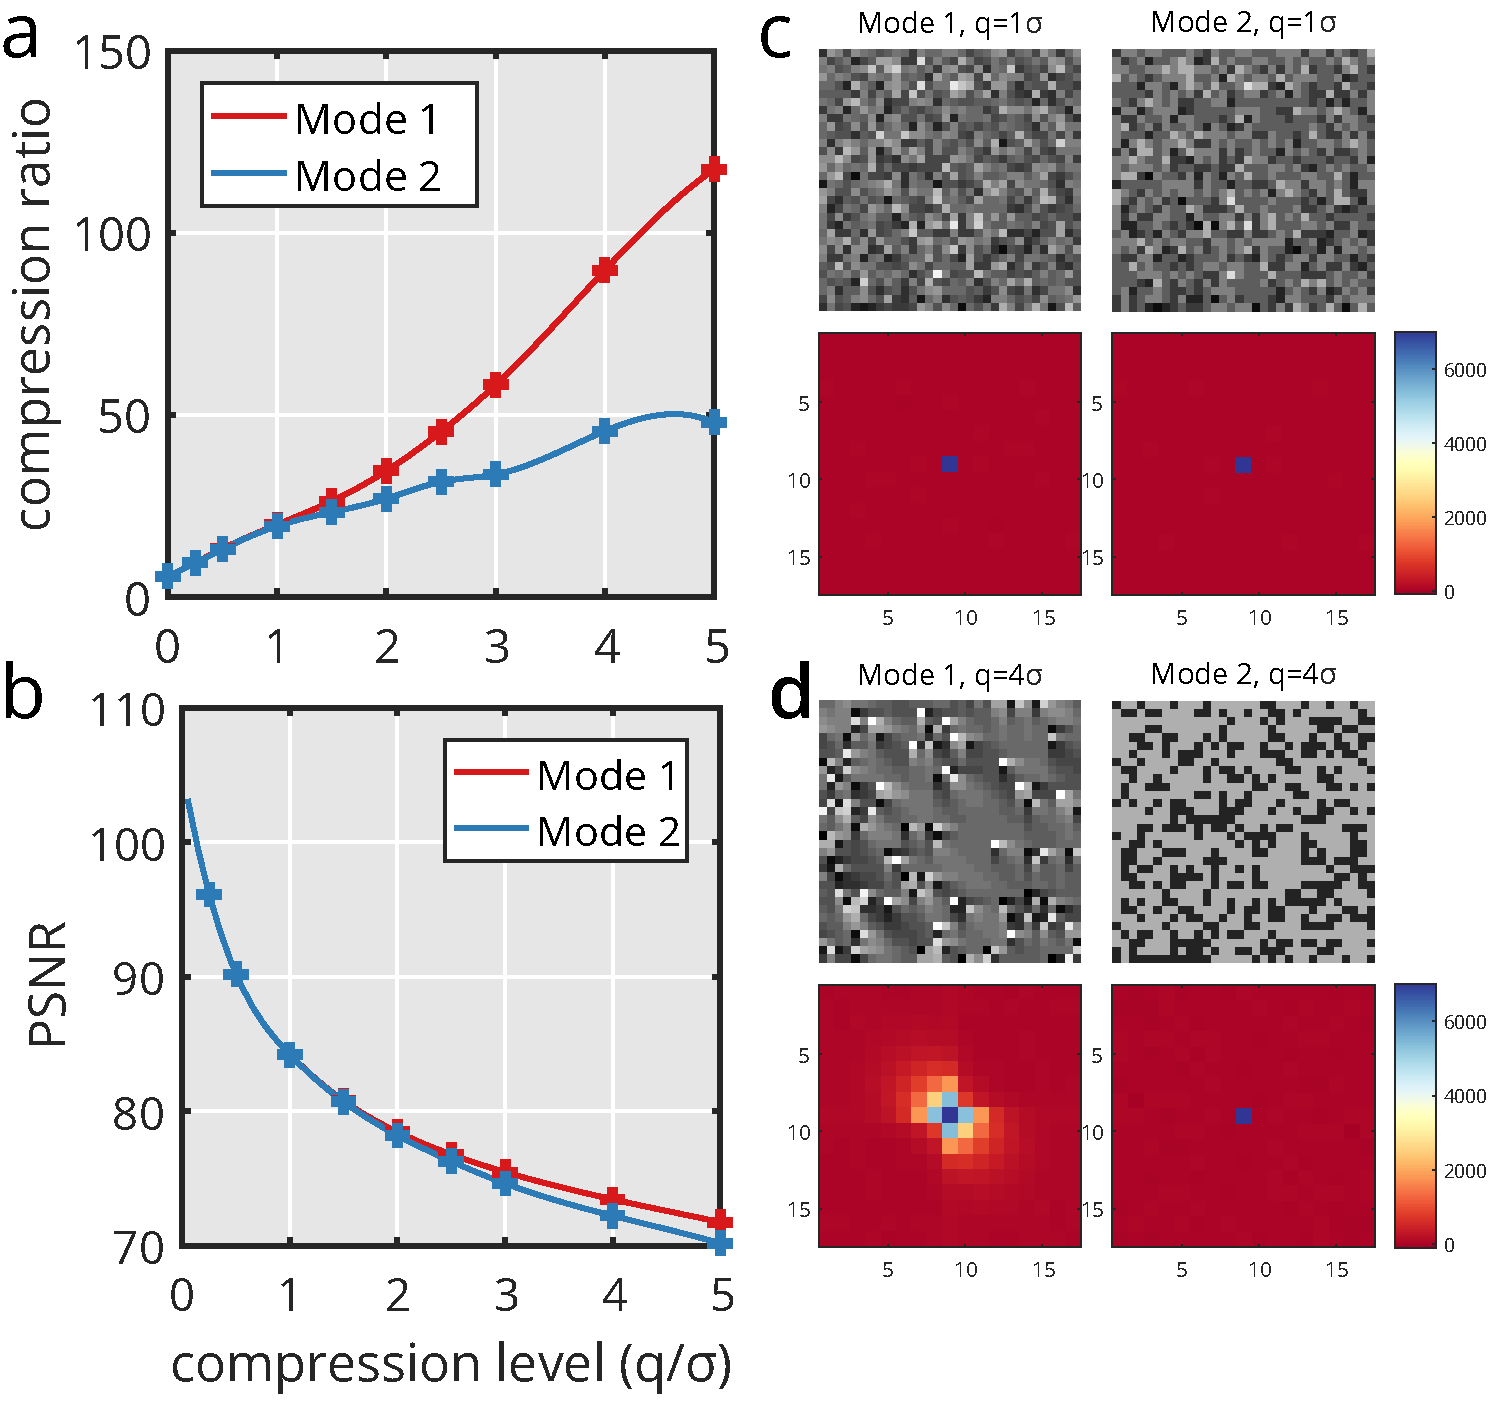
\includegraphics[page=1,width=0.7\textwidth]{swapping}
      \bcaption[Options for noise dependent lossy compression]{Comparing Mode 1 (prediction then quantization) and Mode 2 (quantization then prediction) of noise dependent lossy compression in terms of compression ratio, peak signal to noise ratio (PSNR) and spatial correlations introduced to random noise. (\textbf{a}) Compression ratio as a function of the quantization step for Mode 1 and Mode 2. (\textbf{b}) PSNR as a function of the quantization step for Mode 1 and Mode 2. (\textbf{c, d}) Random noise was compressed at various quantization steps both for Mode 1 and Mode 2. Autocorrelation was calculated for the compressed images to see whether the compression introduces any spatial correlation between the pixels. For q=1$\upsigma$ both modes are free of correlation (\textbf{c}, top: compressed images, bottom: autocorrelation), however, for q=2$\upsigma$ Mode 1 exhibits a correlation pattern (\textbf{d}, top left: compressed image, bottom left: autocorrelation) that is not present in Mode 2 (\textbf{d}, top right compressed image, bottom right: autocorrelation). For more discussion, see "\textbf{Supplementary Note}".}
      \label{fig:swapping}
    \end{figure}

  \subsection{Benchmarking}

    \begin{figure}[tpb]
      \centering
      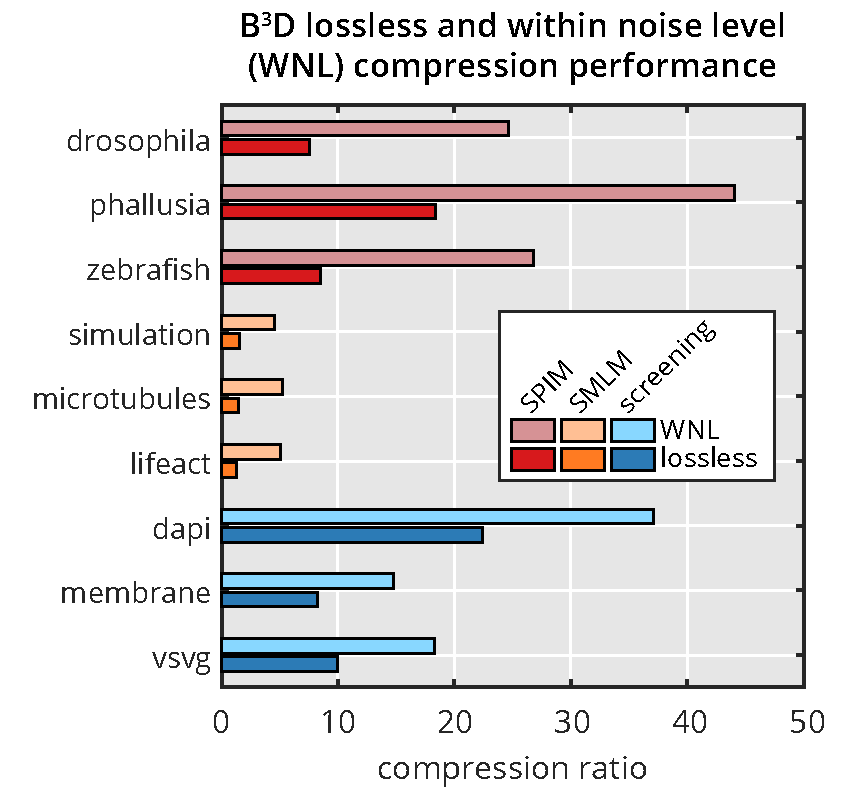
\includegraphics[page=1,height=0.5\textwidth]{Fig1c_compressionBars}
      \bcaption[Within noise level compression performance]{WNL compression performance compared with lossless performance for 9 different dataset representing 3 imaging modalities (SPIM, SMLM, screening). Compression ratio = original size / compressed size. For description of datasets see Table \ref{tab:datasets} in Appendix B.}
      \label{fig:benchmark}
    \end{figure}

    \begin{figure}[tpb]
      \centering
      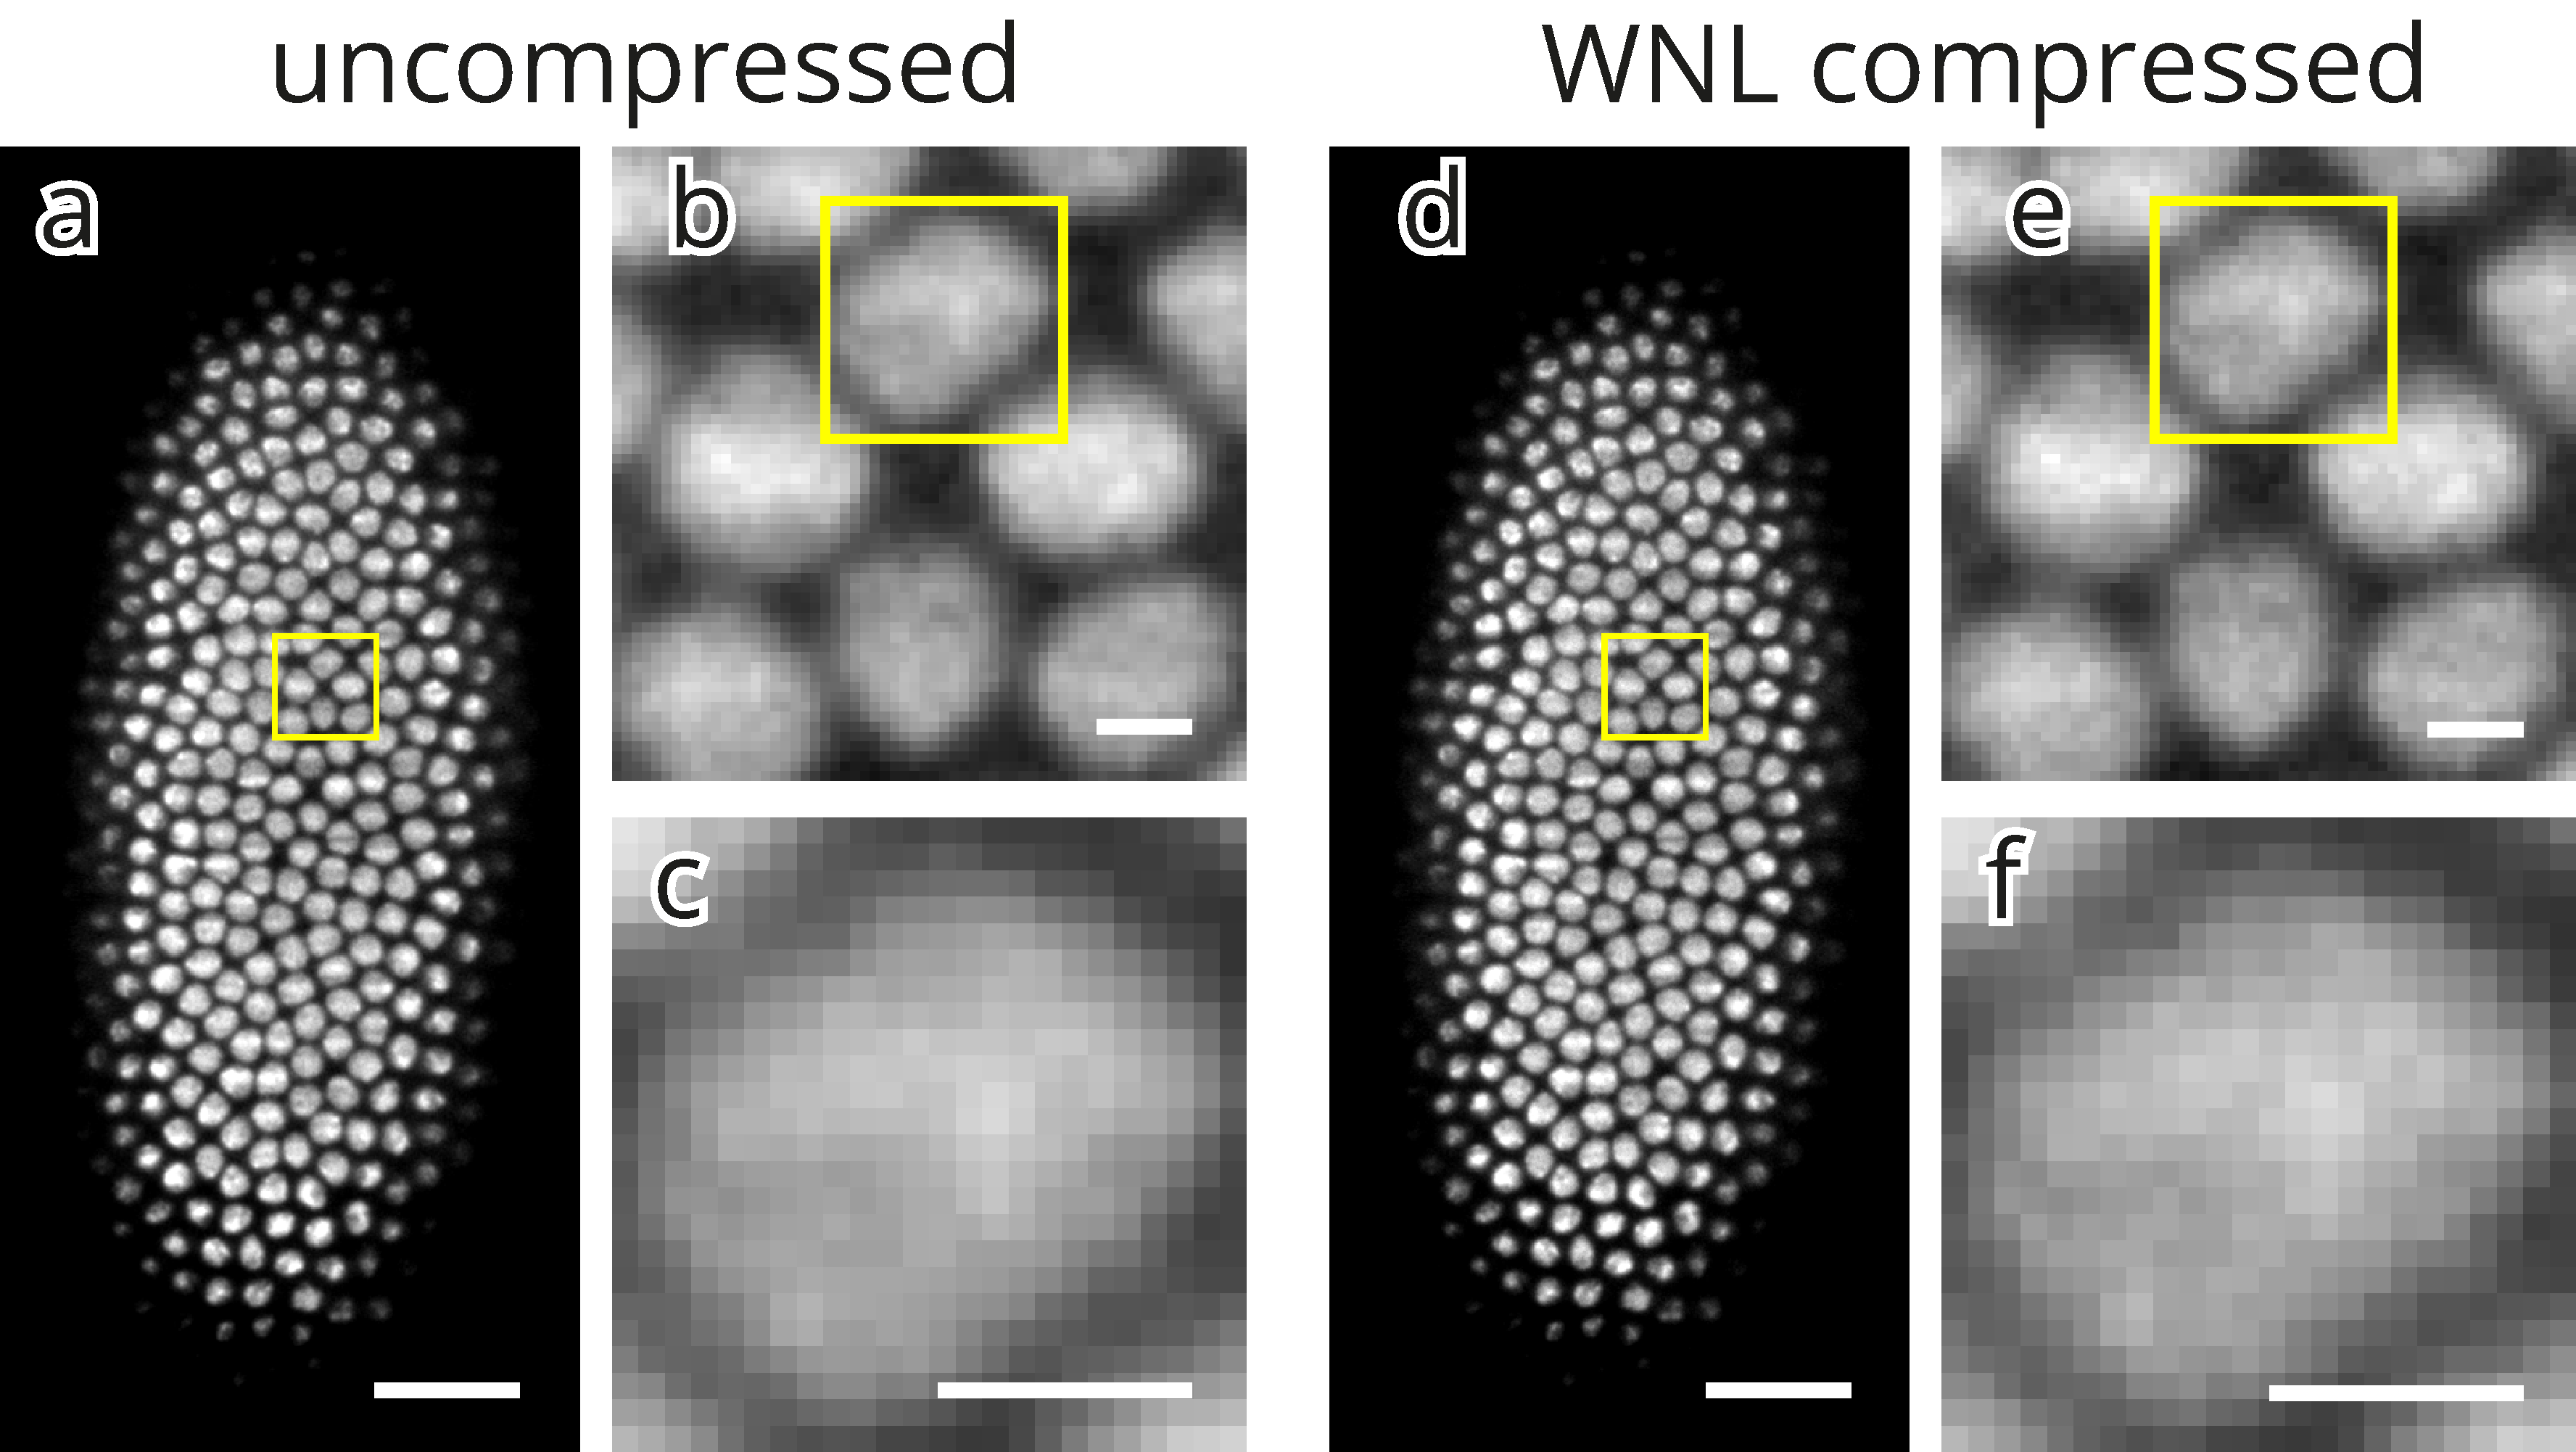
\includegraphics[page=1,width=0.9\textwidth]{wnlSamples}
      \bcaption[Image quality of a WNL compressed dataset]{WNL compression performance compared with lossless performance for 9 different dataset representing 3 imaging modalities (SPIM, SMLM, screening). Compression ratio = original size / compressed size. For description of datasets see Table \ref{tab:datasets}.}
      \label{fig:wnlSamples}
    \end{figure}

    \begin{figure}[tpb]
      \centering
      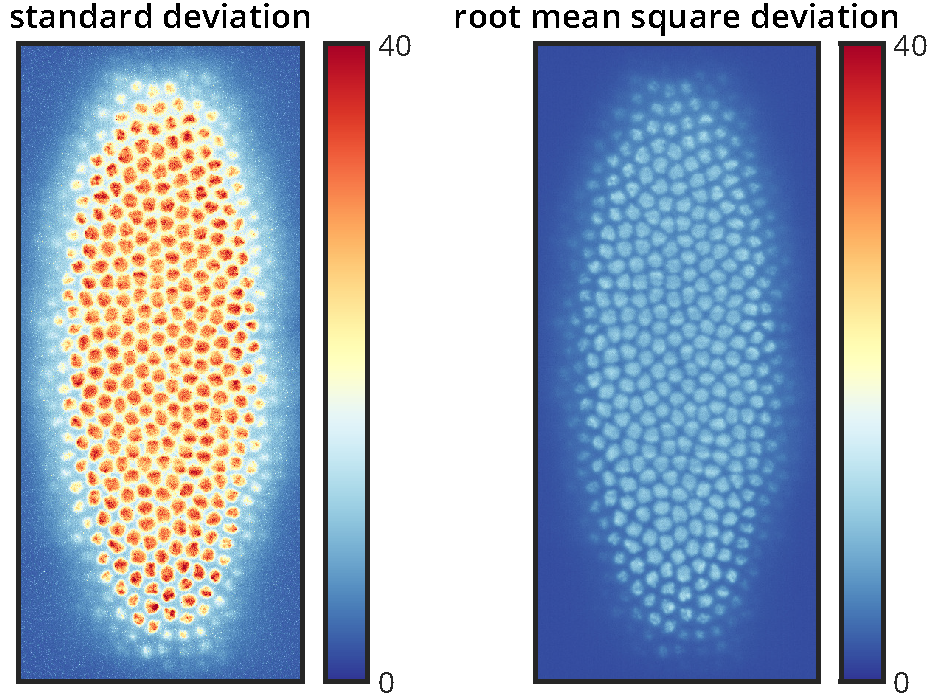
\includegraphics[page=1,width=0.7\textwidth]{SFig4_RMSDvsSD}
      \bcaption[Compression error compared to image noise]{To compare the difference arising from WNL compression to image noise, we imaged a single plane 100 times in a \textit{Drosophila melanogaster} embryo expressing H2Av-mCherry nuclear marker at \SI{38}{ms} intervals. The whole acquisition took \SI{3.8}{s}, for which the sample can be considered stationary. To visualize image noise, the standard deviation was calculated for the uncompressed images (left). All images were then WNL compressed, and the root mean square deviation was calculated compared to the uncompressed images (right). The root mean square deviation on average is 3.18 times smaller than the standard deviation of the uncompressed images.}
      \label{fig:RMSD}
    \end{figure}

    

    \begin{figure}[tpb]
      \centering
      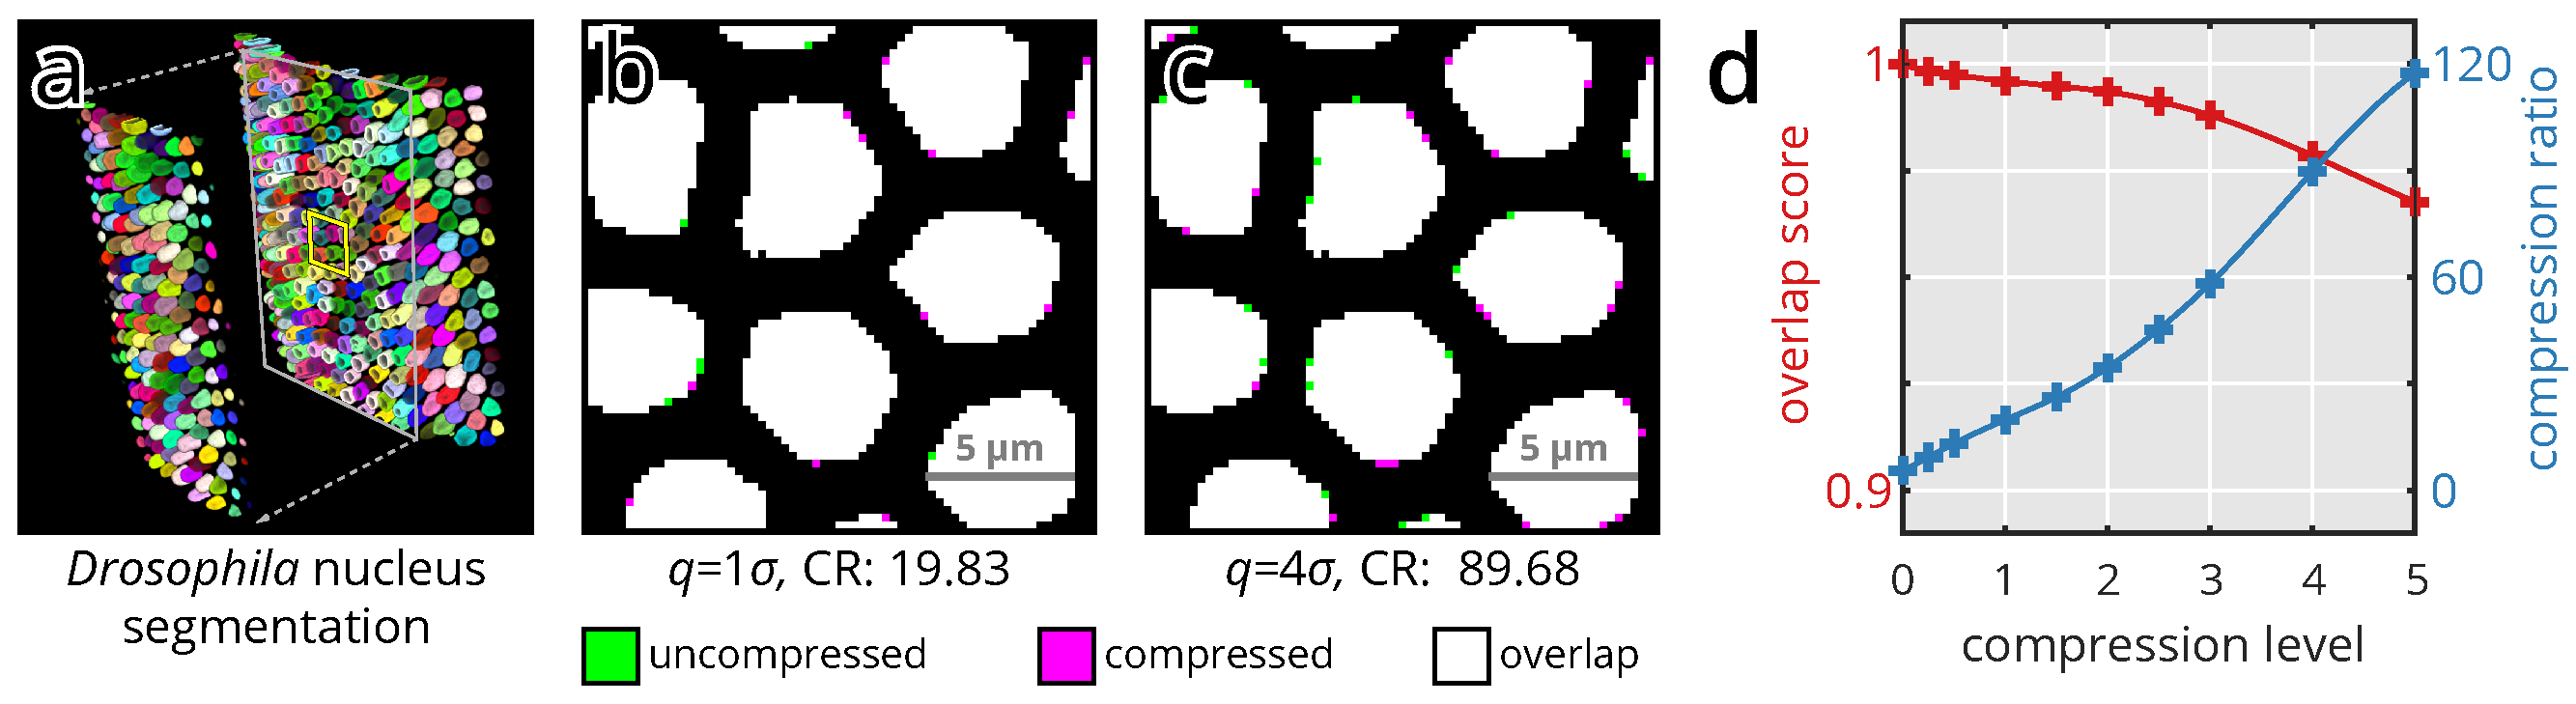
\includegraphics[page=1,width=1\textwidth]{LLvsB3D}
      \bcaption[Influence of noise dependent lossy compression on 3D nucleus segmentation]{A \textit{Drosophila melanogaster} embryo expressing H2Av-mCherry nuclear marker was imaged in MuVi-SPIM \cite{krzic_multiview_2012}, and 3D nucleus segmentation was performed ( "\textbf{Online Methods}") (\textbf{a}). The raw data was subsequently compressed at increasingly higher compression levels, and segmented based on the training of the uncompressed data. To visualize segmentation mismatch, the results of the uncompressed (green) and compressed (magenta) datasets are overlaid in a single image (\textbf{b}, \textbf{c}; overlap in white). Representative compression levels were chosen at two different multiples of the photon shot noise, at q=1$\upsigma$ (\textbf{b}) and q=4$\upsigma$ (\textbf{c}). For all compression levels the segmentation overlap score ( "\textbf{Online Methods}") was calculated and is plotted in (\textbf{g}) along with the achieved compression ratios.}
      \label{fig:wnlDroso}
    \end{figure}

    \begin{figure}[tpb]
      \centering
      \includegraphics[page=3,width=1\textwidth]{LLvsB3D}
      \bcaption[Influence of noise dependent lossy compression on 3D membrane segmentation]{A \textit{Phallusia mammillata} embryo expressing PH-citrine membrane marker was imaged in MuVi-SPIM \cite{krzic_multiview_2012}, and 3D membrane segmentation was performed ( "\textbf{Supplementary Methods}") (\textbf{a}). The raw data was subsequently compressed at increasingly higher compression levels, and segmented using the same settings as the uncompressed data. To visualize segmentation mismatch, the results of the uncompressed (green) and compressed (magenta) datasets are overlaid in a single image (\textbf{b, c}; overlap in white). Representative compression levels were chosen at two different multiples of the photon shot noise, at q=1.6$\upsigma$ (\textbf{b}) and q=4.8$\upsigma$ (\textbf{c}). For all compression levels the segmentation overlap score ( "\textbf{Supplementary Methods}") was calculated and is plotted in (\textbf{d}) along with the achieved compression ratios.}
      \label{fig:wnlPhallusia}
    \end{figure}

    \begin{figure}[tpb]
      \centering
      \includegraphics[page=2,width=1\textwidth]{LLvsB3D}
      \bcaption[Influence of noise dependent lossy compression on single-molecule localization]{Microtubules, immunolabeled with Alexa Fluor 647 were imaged by SMLM (\textbf{a}). The raw data was compressed at increasingly higher compression levels, and localized using the same settings as the uncompressed data. To visualize localization mismatch, the results of the uncompressed (green) and compressed (magenta) datasets are overlaid in a single image (\textbf{b}, \textbf{c}; overlap in white). Two representative compression levels were chosen at q=1$\upsigma$ (\textbf{b}) and q=4$\upsigma$ (\textbf{c}). To assess the effects of compression on localization precision, a simulated dataset with known emitter positions was compressed at various levels. For all compression levels the relative localization error (normalized to the Cramér–Rao lower bound) was calculated and is plotted in (\textbf{d}) along with the achieved compression factors.}
      \label{fig:wnlSMLM}
    \end{figure}

    \begin{figure}[tpb]
      \centering
      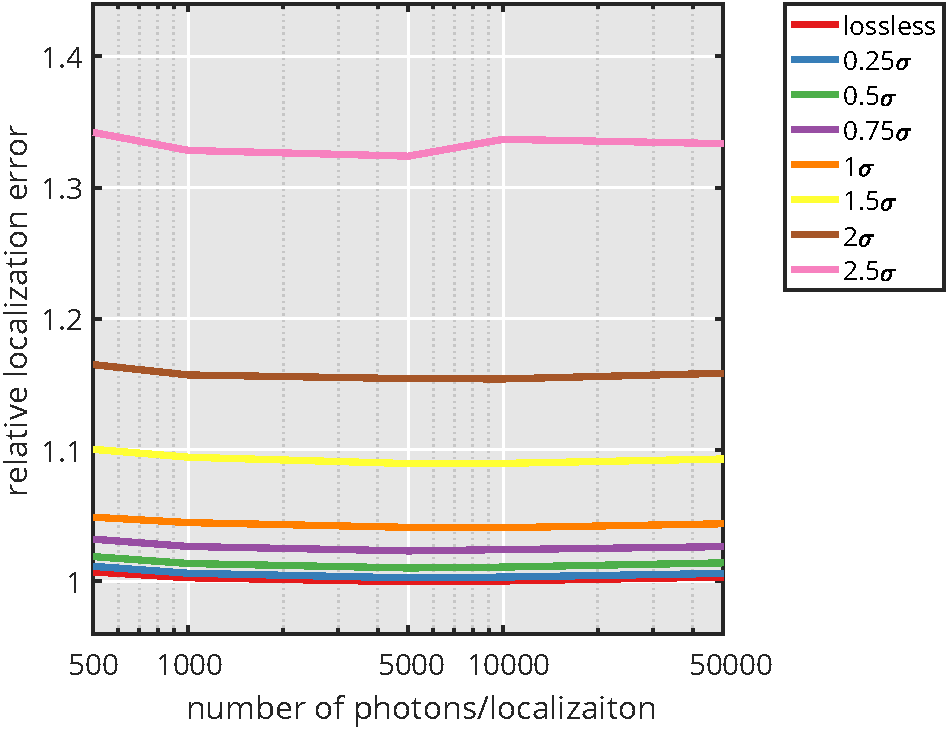
\includegraphics[page=1,width=0.5\textwidth]{SFig6_locprecVsNphotons}
      \bcaption[Change in localization error only depends on selected quantization step]{We simulated multiple datasets ( "\textbf{Supplementary Methods}") with different average photon numbers per localization. Background was kept at a constant average of 20 photons/pixel. Datasets were compressed at multiple compression levels (see legend), and localization error relative to the Cramér-Rao lower bound was calculated. The relative localization error only depends on the compression level, and not on the signal to background illumination ratio.}
      \label{fig:SFig6_locprecVsNphotons}
    \end{figure}



\section{Noise dependent lossy compression}
  
  square root compression \cite{gowen_square_2003}
  noise and bias in square root compression \cite{bernstein_noise_2010}
  quantization \cite{gray_quantization_1998}
  Anscombe \cite{anscombe_transformation_1948}
  optimal inverse Anscombe \cite{makitalo_optimal_2011,makitalo_closed-form_2011}
  optimal inverse generalized Anscombe \cite{makitalo_optimal_2013}

\section{Methods}
  
\subsubsection{Compression benchmarking}
For all presented benchmarks, TIFF and JPEG2000 performance was measured through MATLAB's imwrite and imread functions, while KLB and \b3d performance was measured in C++. All benchmarks were run on a computer featuring 32 processing cores (2×Intel Xeon E5-2620 v4), \SI{128}{GB} RAM and an NVIDIA GeForce GTX 970 graphics processing unit. Read and write measurements were performed in RAM to minimize I/O overhead, and are an average of 5 runs.

\subsubsection{Light-sheet imaging}
\textit{Drosophila} embryos were imaged in our MuVi-SPIM setup \cite{krzic_multiview_2012} using the electronic confocal slit detection (eCSD) \cite{de_medeiros_confocal_2015}. Embryos were collected on an agar juice plate, and dechorionated in 50\% bleach solution for \SI{1}{min}. The embryos were then mounted in a shortened glass capillary (Brand \SI{100}{\micro l}) filled with 0.8\% GelRite (Sigma-Aldrich), and pushed out of the capillary to be supported only by the gel.

\subsubsection{3D nucleus segmentation}
3D nucleus segmentation of \textit{Drosophila} embryos was performed using Ilastik \cite{sommer_ilastik:_2011}. The original dataset was compressed at different quantization levels, then upscaled in z to obtain isotropic resolution. To identify the nuclei, we used the pixel classification workflow, and trained it on the uncompressed dataset. This training was then used to segment the compressed datasets as well. Segmentation overlap was calculated in Matlab ( "Supplementary Code") using the Sørensen–Dice index \cite{sorensen_method_1948,dice_measures_1945}:
\begin{equation}
  QS = 2 \left| A \cap B \right| / \left( |A| + |B| \right)
\end{equation}
where the sets $A$ and $B$ represent the pixels included in two different segmentations.

\subsubsection{3D membrane segmentation}
Raw MuVi-SPIM recordings of \textit{Phallusia mammillata} embryos expressing PH-citrine membrane marker were kindly provided by Ulla-Maj Fiuza (EMBL, Heidelberg). Each recording consisted of 4 views at 90 degree rotations. The views were fused using an image based registration algorithm followed by a sigmoidal blending of the 4 views. The fused stack was then segmented using the MARS algorithm \cite{fernandez_imaging_2010} with an hmin parameter of 10. The raw data (all 4 views) was compressed at different levels, and segmented using the same pipeline. Segmentation results were then processed in Matlab to calculate the overlap score for the membranes using the Sørensen–Dice index ( "Supplementary Code").

\subsubsection{Single-molecule localization imaging}
In order to visualize microtubules, U2OS cells were treated as in \cite{deschamps_3d_2014} and imaged in a dSTORM buffer \cite{heilemann_subdiffraction-resolution_2008}. In brief, the cells were permeabilized and fixed with glutaraldehyde, washed, then incubated with primary tubulin antibodies and finally stained with Alexa Fluor 647 coupled secondary antibodies. The images were recorded on a home-built microscope previously described \cite{deschamps_3d_2014}, in its 2D single-channel mode.

\subsubsection{Single-molecule localization data analysis}
Analysis of single-molecule localization data was performed on a custom-written MATLAB software as in \cite{deschamps_efficient_2016}. Pixel values were converted to photon counts according to measured offset and calibrated gain of the camera (EMCCD iXon, Andor). The background was estimated with a wavelet filter \cite{izeddin_wavelet_2012}, background-subtracted images were thresholded and local maxima were detected on the same images. 7-pixel ROIs around the detected local maxima were extracted from the raw images and fitted with a GPU based MLE fitter \cite{smith_fast_2010}. Drift correction was performed based on cross-correlation. Finally, images were
reconstructed by filtering out localizations with a high uncertainty (>\SI{30}{nm} and large PSF (>\SI{150}{nm}) and Gaussian rendering.

\subsubsection{Simulation of single-molecule localization data}
Single molecule localization data was simulated in Matlab ( "Supplementary Code") by generating a grid of pixelated Gaussian spots with standard deviation of 1 pixel. With a pixel size of a 100 nm, this corresponds to a FWHM of 235.48 nm. The center of each spot was slightly offset from the pixel grid at 0.1 pixel increments in both x and y directions. To this ground truth image a constant value was added for illumination background, and finally Poisson noise was applied to the image. This process was repeated 10000 times to obtain enough images for adequate accuracy.

\subsubsection{Code availability}
Code used for analyzing data, \b3d source code and compiled binaries, including a filter plugin for HDF5, is available for download at https://git.embl.de/balazs/B3D.
